%Copyright (c) 2014 Gabi Sarkis <gfsarkis@gmail.com>
% 
%Permission is hereby granted, free of charge, to any person obtaining a copy
%of this software and associated documentation files (the "Software"), to deal
%in the Software without restriction, including without limitation the rights
%to use, copy, modify, merge, publish, distribute, sublicense, and/or sell
%copies of the Software, and to permit persons to whom the Software is
%furnished to do so, subject to the following conditions:
% 
%The above copyright notice and this permission notice shall be included in
%all copies or substantial portions of the Software.
% 
%THE SOFTWARE IS PROVIDED "AS IS", WITHOUT WARRANTY OF ANY KIND, EXPRESS OR
%IMPLIED, INCLUDING BUT NOT LIMITED TO THE WARRANTIES OF MERCHANTABILITY,
%FITNESS FOR A PARTICULAR PURPOSE AND NONINFRINGEMENT. IN NO EVENT SHALL THE
%AUTHORS OR COPYRIGHT HOLDERS BE LIABLE FOR ANY CLAIM, DAMAGES OR OTHER
%LIABILITY, WHETHER IN AN ACTION OF CONTRACT, TORT OR OTHERWISE, ARISING FROM,
%OUT OF OR IN CONNECTION WITH THE SOFTWARE OR THE USE OR OTHER DEALINGS IN
%THE SOFTWARE.


\documentclass[table]{beamer}
\usepackage{tikz}
\usepackage{verbatim}
\setbeamertemplate{bibliography item}{\insertbiblabel}
\usepackage[style=ieee,
% citestyle=numeric, %define style for citations
    % bibstyle=abbrv, %define style for bibliography
    % maxbibnames=10, %maximum number of authors displayed in bibliography
    % minbibnames=1, %minimum number of authors displayed in bibliography
    % maxcitenames=3, %maximum number of authors displayed in citations before using et al.
    % minnames=1, %maximum number of authors displayed in citations before using et al.
    datezeros=false, % do not print dates with leading zeros
    date=long, %use long formats for dates
    isbn=false,% show no ISBNs in bibliography (applies only if not a mandatory field)
    url=false,% show no urls in bibliography (applies only if not a mandatory field)
    doi=false, % show no dois in bibliography (applies only if not a mandatory field)
    eprint=false, %show no eprint-field in bibliography (applies only if not a mandatory field)
    backend=bibtex %use biber as the backend; backend=bibtex is less powerful, but easier to install
    ]{biblatex}

\usepackage[utf8]{inputenc}
\usepackage{palatino}
\usepackage{graphicx}
\graphicspath{ {images/} }
\usepackage[labelfont=bf]{caption}
\usepackage{float}
\usepackage{subcaption}
\usepackage{setspace}
\captionsetup[table]{font = {stretch=1.35}}
\captionsetup[figure]{font = {stretch=1.35}}
\usepackage[margin=1in]{geometry}
\usepackage{tabularx}
\usepackage{booktabs}
\usepackage{multirow}
\usepackage[table,xcdraw]{xcolor} %colors in table
\usepackage{amsmath,amssymb}
\usepackage{mathtools}
\usepackage{bbm}
\usepackage{afterpage}

\usetikzlibrary{arrows,shapes,backgrounds}

\mode<presentation>{

\definecolor{bluecern}{HTML}{0053A1}

\usetheme{Frankfurt}

\setbeamercolor{structure}{fg=titlecolors}
\setbeamercolor{subsection in head/foot}{bg=titlecolor}
}

% \setbeamercolor{title}{bg=white, fg=red}
% \setbeamercolor{frametitle}{bg=white, fg=red}
% \setbeamercolor{section in head/foot}{fg=black, bg=white}
\colorlet{LightSpringGreen}{white!70!black}
\setbeamercolor{section in head/foot}{fg=white, bg=LightSpringGreen}

% set bullet color on progress bar
\colorlet{bullet}{green}
\defbeamertemplate*{mini frame}{Frankfurt}
{%
  \begin{pgfpicture}{0pt}{0pt}{0.1cm}{0.1cm}
%    \pgfsetcolor{bullet}% draw and fill in red
    \pgfsetfillcolor{bullet}% only fill in red
    \pgfpathcircle{\pgfpoint{0.05cm}{0.05cm}}{0.05cm}
    \pgfusepath{fill,stroke}
  \end{pgfpicture}%
}
[action]
{ \setbeamersize{mini frame size=.14cm,mini frame offset=.03cm} }


\usetheme{mcgill}

\setcounter{tocdepth}{1}

\title[Haptic Tacton Similarity]{Haptic Tacton Perceptual Similarity} %what is inside the [] appears at the bottom of every page
\subtitle[]{(cooler title still TBD)}
\author[Marc Demers]{Marc~Demers}
\institute[McGill University]
{
  \inst{}%
  McGill University, Montr\'{e}al, QC.
}

\date[]{\today}

%kl-div
\DeclarePairedDelimiterX{\infdivx}[2]{(}{)}{%
  #1\;\delimsize\|\;#2%
}
\newcommand{\infdiv}{D_{KL}\infdivx}
\DeclarePairedDelimiter{\norm}{\lVert}{\rVert}

\newcommand\given[1][]{\:#1\vert\:}

\bibliography{references,zotero-references}

\begin{document}
% For every picture that defines or uses external nodes, you'll have to
% apply the 'remember picture' style. To avoid some typing, we'll apply
% the style to all pictures.
\tikzstyle{every picture}+=[remember picture]
\tikzstyle{na} = [baseline=-.5ex]

\frame[plain]{
  \titlepage
}

\section{Intro} %defines the top level presentation title

\begin{frame}{Objective}

  \begin{itemize}
  \item Present project to newcomers
  \item Present results
  \item Ideas for data analysis
  \item Kickstart writing paper (find appropriate venue)
  
  \end{itemize}

\end{frame}

%%%%


\begin{frame}{Quick Intro}
    
    \begin{itemize}
        \item Haptics: the sense of touch
        \item Tacton: \textit{Tactile Icon}
        \item Structured abstract tactile messages that encode information that can be carried non-visually, usually via tactile encoding or via force.
        \item The design of tactons is typically left to an ``expert'' although there are some libraries that contain a lexicality
        \item This lengthy design process hinders development of haptic technologies both on the research-side and the consumer side
        \item We focus on Vibrotactile (VT) tactons that are \texit{binary} (ON/OFF)
    \end{itemize}
    
\end{frame}



\begin{frame}{Motivation \& Challenges}

  
  \begin{itemize}
      \item Countless papers run user studies to find parameters that influence our perception of tactons, but reinvent the wheel on each iteration
      \item Need for characterizing Individual Differences (IDs) in our perception of tactons
      \item Only a subset of the tacton space is explored on every iteration, making scalability difficult
      \item Generating tactons that elicit certain responses from the user is the next logical step, but very little is currently known from our \textit{perception} of tactons
  \end{itemize}


\end{frame}


\begin{frame}{Research Question}
    
    \begin{itemize}
        \item Can we predict the perceptual similarity of VT tactons?
        \begin{itemize}
            \item How to do it efficiently across the whole space of tactons (of vibrations)
            \item How to conduct user studies for haptics in a remote environment such as crowdsourcing platforms
        \end{itemize}
    
        \item Investigate the perceptual similarity of haptics \textit{across users}. This relates to the idea of \textit{personalizing} the stimuli.
    \end{itemize}
    
\end{frame}



\begin{frame}{Contributions}
        
    \begin{enumerate}
        \item We develop an Android application for smartphones that can render VT stimuli and gather feedback about them.
        \item We gather large amounts of feedback in a crowdsourced setting, via Amazon Mechanical Turk~\footnote{https://www.mturk.com/} (AMT).
        \item We apply our graph theoretic methodology to analyzing the data.
        \item We use a hold-out set to predict similarity between never-seen-before tacton pairs in the graph.
    \end{enumerate}
    
\end{frame}






\section{Approach}


\begin{frame}{Theoretical Approaches for Measuring Similarity}

\begin{table}[htbp]\small
\centering
\resizebox{0.9\textwidth}{!}{
    \begin{tabular}{lcccl}
     &  & \multicolumn{2}{c}{Decision Process} &  \\ \cline{3-4}
     & \multicolumn{1}{c|}{} & \multicolumn{1}{c|}{Deterministic} & \multicolumn{1}{c|}{Probabilistic} &  \\ \cline{2-4}
    \multicolumn{1}{c|}{\multirow{2}{*}{Percept}} & \multicolumn{1}{c|}{Deterministic} & \multicolumn{1}{c|}{\begin{tabular}[c]{@{}c@{}}Type 0\\ MDS\end{tabular}} & \multicolumn{1}{c|}{\begin{tabular}[c]{@{}c@{}}Type II\\ Logistic\end{tabular}} &  \\ \cline{2-4}
    \multicolumn{1}{c|}{} & \multicolumn{1}{c|}{Probabilistic} & \multicolumn{1}{c|}{\begin{tabular}[c]{@{}c@{}}Type I\\ Classical Thurstonian psychophysics~\cite{thurstone_law_1927}\end{tabular}} & \multicolumn{1}{c|}{\begin{tabular}[c]{@{}c@{}}Type III\\ Probabilistic extensions of Type II models\end{tabular}} &  \\ \cline{2-4}
     & \multicolumn{1}{l}{} & \multicolumn{1}{l}{} & \multicolumn{1}{l}{} &  \\
     & \multicolumn{1}{l}{} & \multicolumn{1}{l}{} & \multicolumn{1}{l}{} & 
    \end{tabular}
}%end resize box
\caption{Classification of similarity psychometric models.}
\label{tab:similarity_psychometrics}
\end{table}


\end{frame}



\begin{frame}{Exploring the Tacton Space}
    \begin{figure}[!htb]
    \centering
    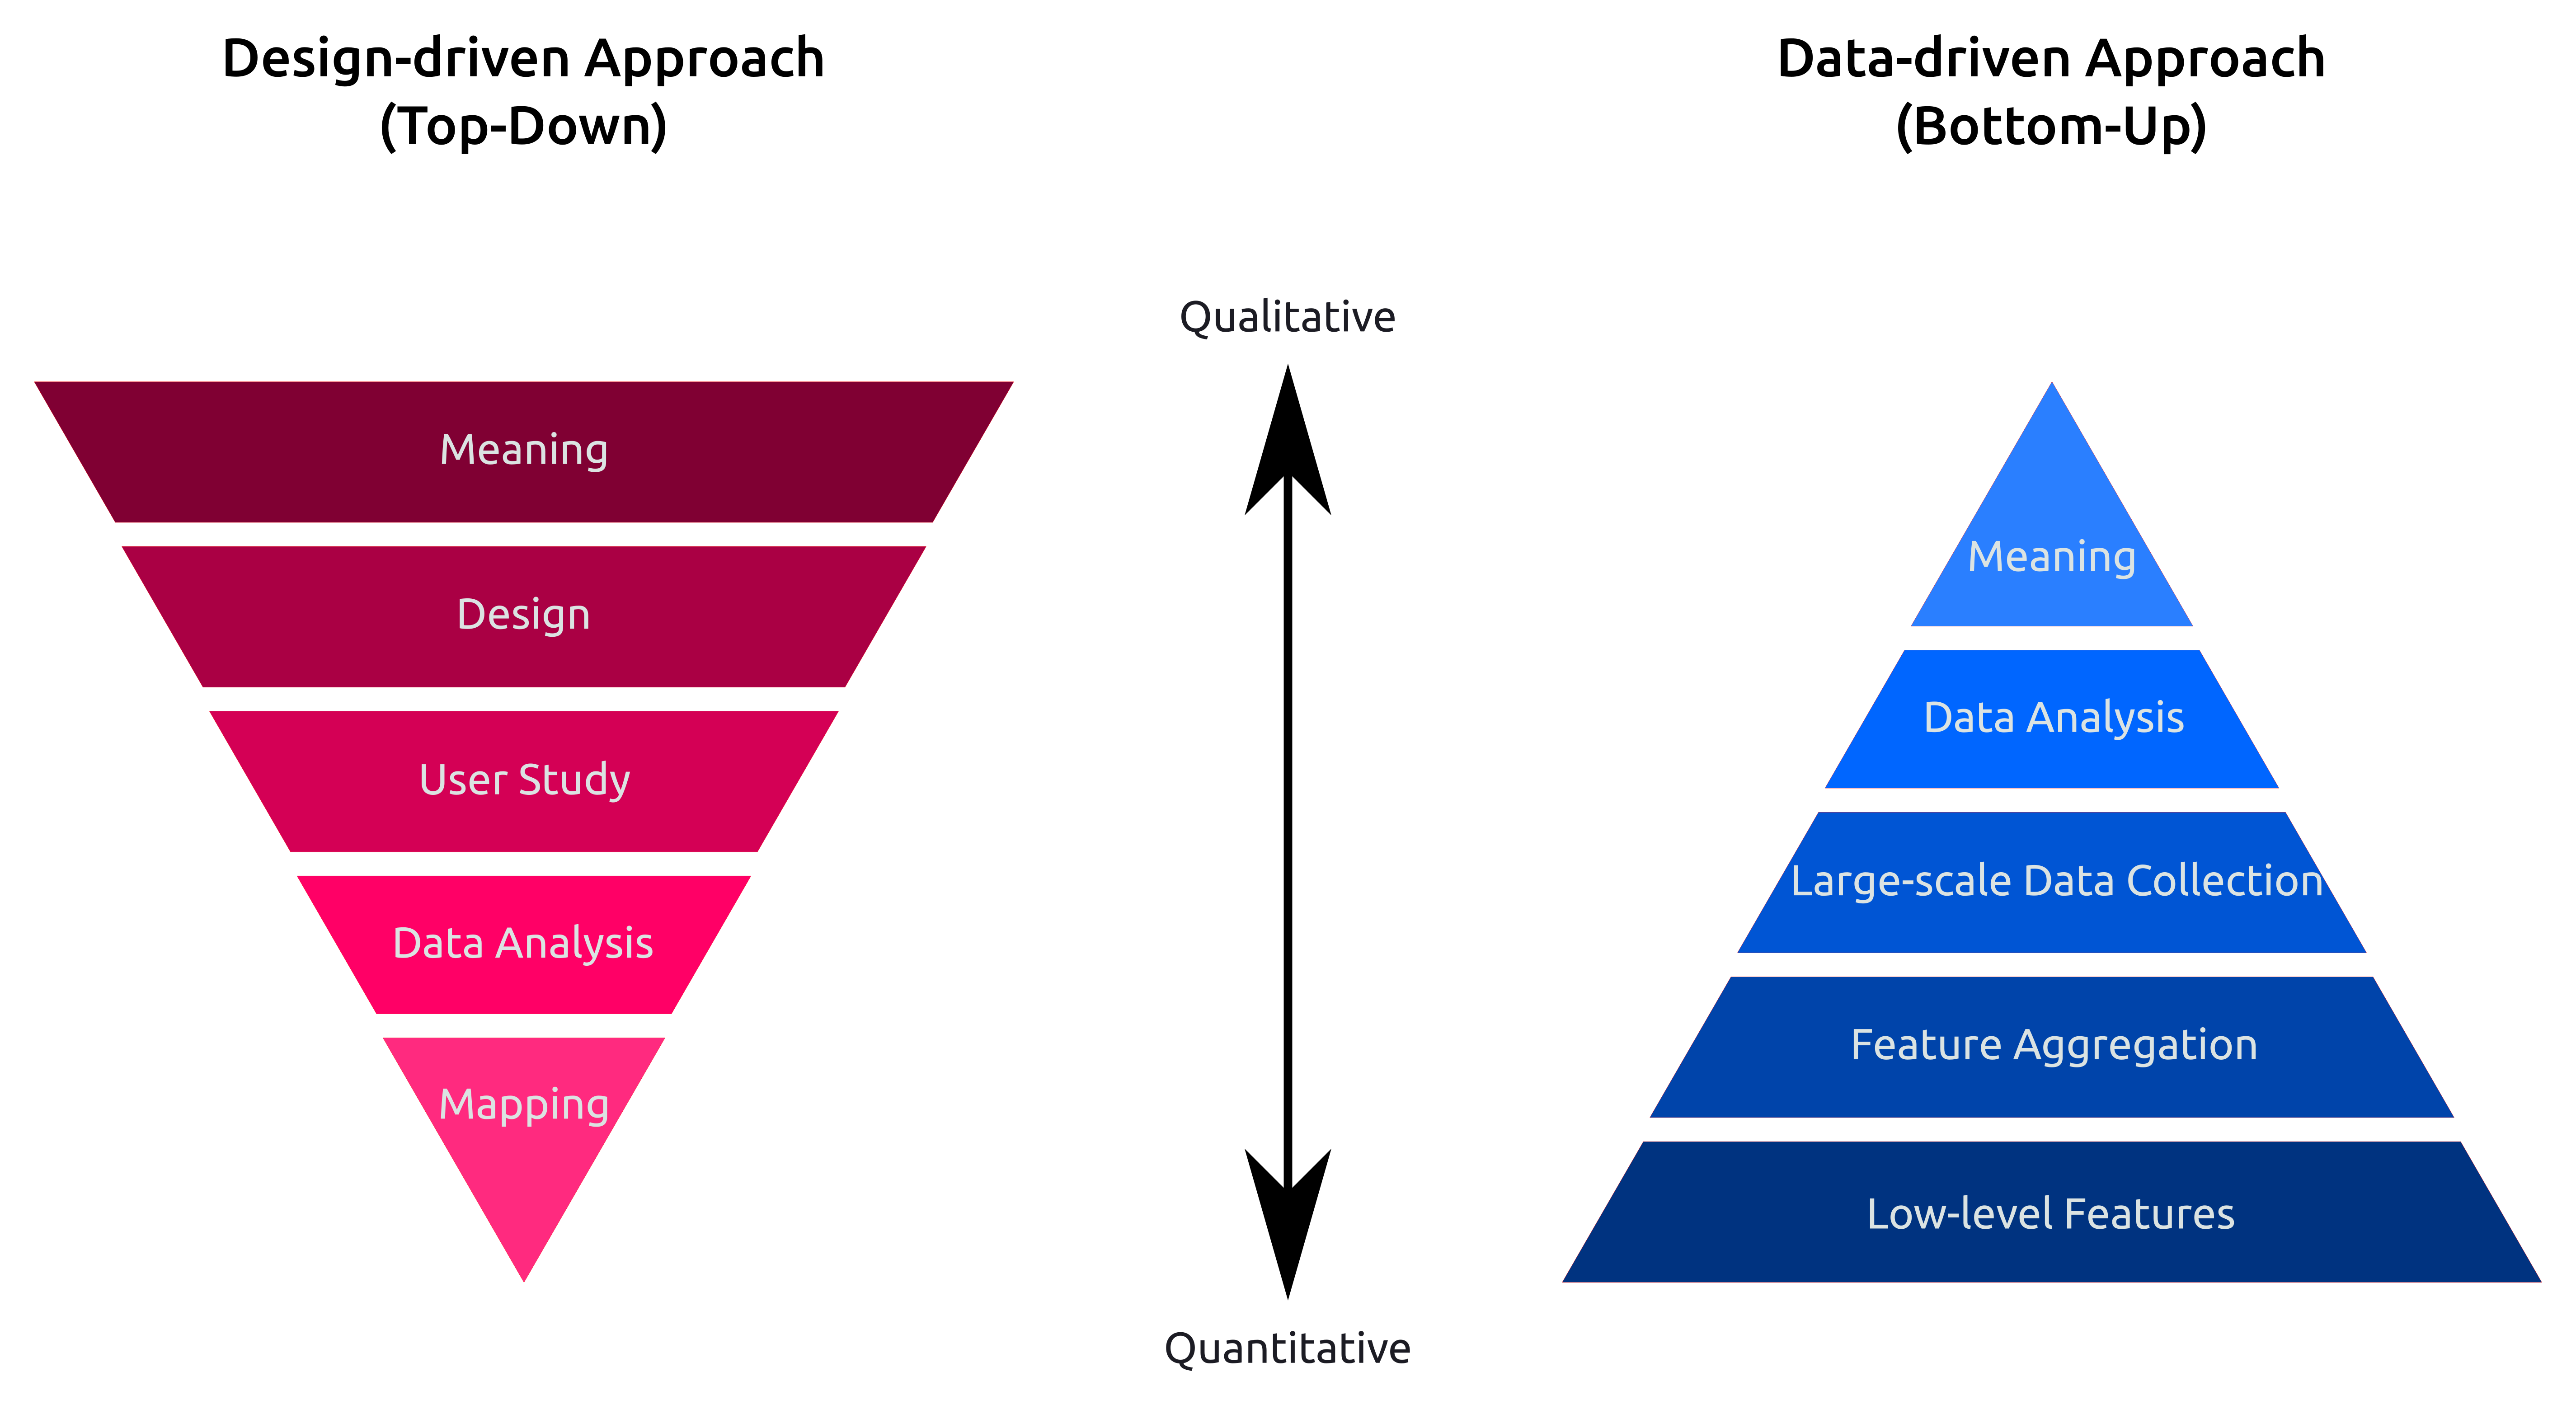
\includegraphics[width=0.8\textwidth,height=\textheight,keepaspectratio]{Images/pyramids.png}
    \end{figure}
\end{frame}




\begin{frame}{Gathering Ratings}

\begin{figure}[!htb]
\centering
\begin{subfigure}{.24\textwidth}
  \centering
  \label{fig:app_process_grouping_1}
  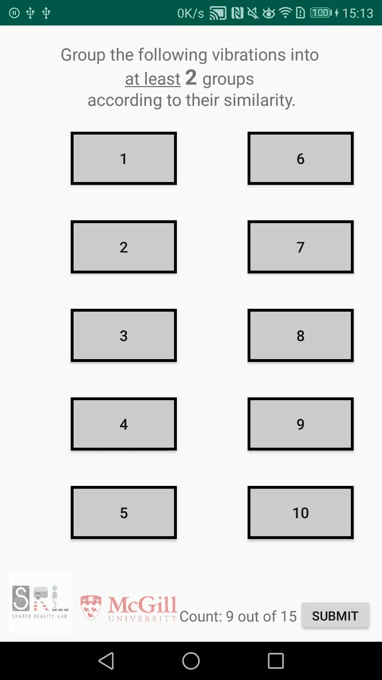
\includegraphics[width=\linewidth]{Images/1.png}
%   \caption{Start of the round.}
\end{subfigure}%
\begin{subfigure}{.24\textwidth}
  \centering
    \label{fig:app_process_grouping_2}
  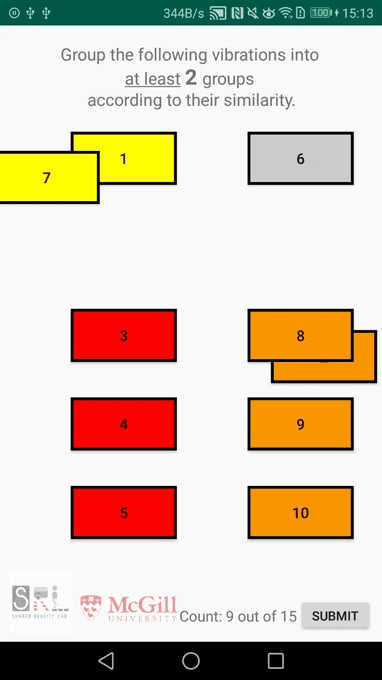
\includegraphics[width=\linewidth]{Images/2.png}
    %  \caption{Evalua\-ting the tactons and iteratively placing them into groups.}
\end{subfigure}
\begin{subfigure}{.24\textwidth}
  \label{fig:app_process_grouping_3}
  \centering
  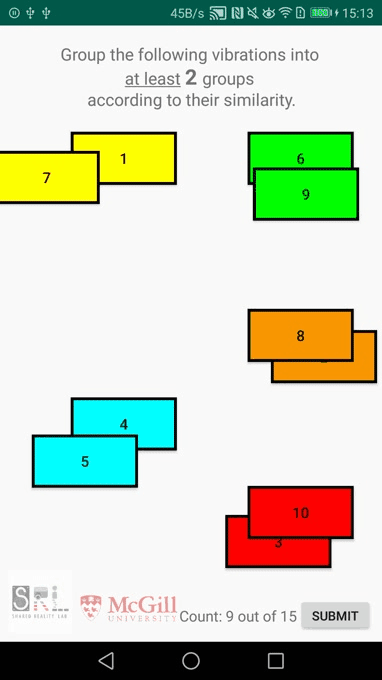
\includegraphics[width=\linewidth]{Images/3.png}
%   \caption{Submitting a grouping.}
\end{subfigure}
\begin{subfigure}{.24\textwidth}
  \centering
  \label{fig:app_process_grouping_4}
  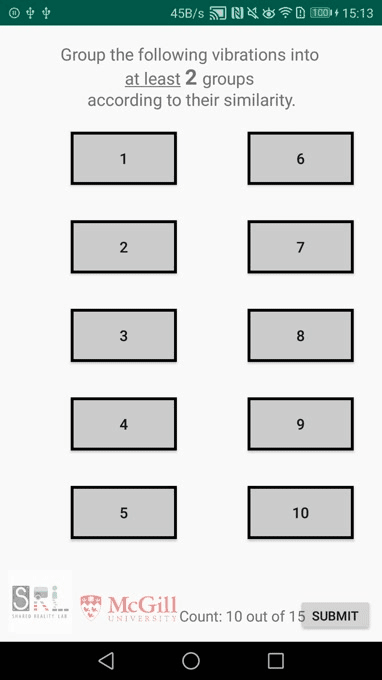
\includegraphics[width=\linewidth]{Images/4.png}
%   \caption{Start of the next round.}
\end{subfigure}
\label{fig:app_process_grouping}
\end{figure}


\end{frame}





\begin{frame}{Probabilistic Modeling}



%source:https://texample.net/tikz/examples/connecting-text-and-graphics/


\begin{columns}

 
    
    \begin{column}{0.48\textwidth}
        Pair Comparison Matrix
        \vspace{1em}
        
        \centering
        \begin{bmatrix}
        0 & 0 & 0 & 0 & 0 & 0 & 1 \tikz[na] \coordinate (s-17); & 0 & 0 & 0 \\ 
          & 0 & 0 & 0 & 0 & 0 & 0 & 1 \tikz[na] \coordinate (s-28); & 0 & 0  \\ 
        \vdots & \vdots & \vdots & \vdots & \vdots & \vdots & \vdots & \vdots & \vdots & \vdots \\
         &  &  &  &  &  &  &  & 0 & 0 \\ 
         &  &  &  &  &  &  &  &  & 0 \\ 
        \end{bmatrix}
    \end{column}
    \begin{column}{0.48\textwidth}
        \tikzstyle{background grid}=[draw, black!50,step=.5cm]
        \begin{tikzpicture}%[show background grid]
            % Put the graphic inside a node. This makes it easy to place the
            % graphic and to draw on top of it. 
            % The above right option is used to place the lower left corner
            % of the image at the (0,0) coordinate. 
            \node [inner sep=0pt,above right] 
                {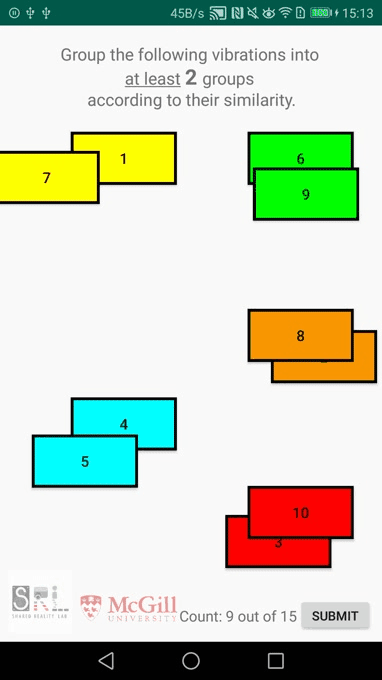
\includegraphics[width=4cm]{Images/3.png}};
            % show origin
            % \fill (0,0) circle (2pt);
            % define destination coordinates
            \path (0.6,5.7) coordinate (im17)
                  (3.0,4.0) coordinate (im28);
        \end{tikzpicture}
    \end{column}
\end{columns}

% define overlays
% Note the use of the overlay option. This is required when 
% you want to access nodes in different pictures.
\begin{tikzpicture}[overlay]
        \path[<-,yellow,thick] (s-17) edge [bend left] (im17);
        \path[<-,orange,thick] (s-28) edge [bend left] (im28);
        % \path[->,blue,thick] (s-cathode) edge [bend left] (cathode);
        % \path[->,red,thick] (s-bridge) edge [out=0, in=-90] (bridge);
\end{tikzpicture}


\end{frame}
\begin{frame}{Probabilistic Modeling}

%source:https://texample.net/tikz/examples/connecting-text-and-graphics/


\begin{columns}
    \begin{column}{0.48\textwidth}
        \centering
        \begin{bmatrix}
        0 &  &  &  &  &  &  &  &  &  \\ 
        0 & 0 &  &  &  &  &  &  &  &  \\ 
        \vdots & \vdots & \vdots & \vdots & \vdots & \vdots & \vdots & \vdots & \vdots & \vdots \\
        1 & 1 & 1 & 1 & 1 & 0 \tikz[na] \coordinate (s-69); & 1 & 1 & 0 &   \\ 
        1 & 1 & 0 \tikz[na] \coordinate (s-310); & 1 & 1 & 1 & 1 & 1 & 1 & 0 \\ 
        \end{bmatrix}
    \end{column}
    \begin{column}{0.48\textwidth}
        \tikzstyle{background grid}=[draw, black!50,step=.5cm]
        \begin{tikzpicture}%[show background grid]
            % Put the graphic inside a node. This makes it easy to place the
            % graphic and to draw on top of it. 
            % The above right option is used to place the lower left corner
            % of the image at the (0,0) coordinate. 
            \node [inner sep=0pt,above right] 
                {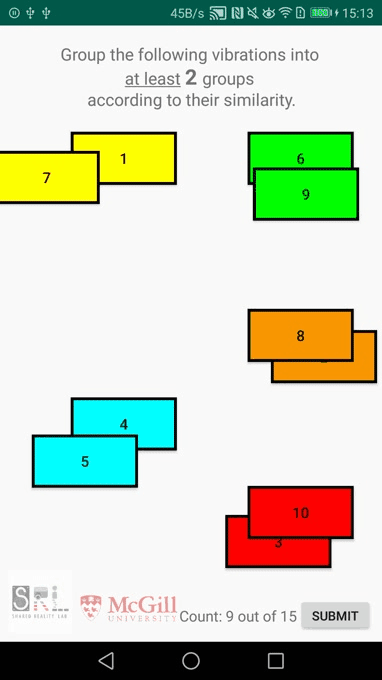
\includegraphics[width=4cm]{Images/3.png}};
            % show origin
            % \fill (0,0) circle (2pt);
            % define destination coordinates
            \path (2.5,5.3) coordinate (im69)
                  (2.3,1.3) coordinate (im310);
        \end{tikzpicture}
    \end{column}
\end{columns}

% define overlays
% Note the use of the overlay option. This is required when 
% you want to access nodes in different pictures.
\begin{tikzpicture}[overlay]
        \path[<-,green,thick] (s-69) edge [bend left] (im69);
        \path[<-,red,thick] (s-310) edge [bend right] (im310);
\end{tikzpicture}


\end{frame}
% \begin{frame}{Probabilistic Modeling}

%source:https://texample.net/tikz/examples/connecting-text-and-graphics/


\begin{columns}
    \begin{column}{0.48\textwidth}
        \centering
        \tiny
        \begin{equation*}
            \tiny
            \label{eqn:gaussian}
            \alpha_{ij} = \sum_{r=0}^{R} \eta^r w_{ij}^r \, y_{ij}^r + \epsilon_{ij}, \qquad \epsilon_{ij} \sim \mathcal{N}(0, \sigma_{ij}^2)
        \end{equation*}
        \begin{equation*}
        \eta^r w_{ij}^r = \eta^r \frac{\text{total num. groups}}{\text{num. similar groups}}, \,  i<j
        \\
        \eta^rw_{ij}^r = \eta^r \frac{\text{total num. groups}}{\text{num. dissimilar groups}}, \,  i>j
        \end{equation*}\\
        \vspace{0.3cm}
        
        %considering that one of the pairs is the attention test we have 10*9/2 FPC, which gives 5 similar pairs and 39 dissimilar pairs. 39+5 = 44, 44+1(attention pair) = 45 =10*9/2
        % idea is to have top and bottom sum up to 1
        % \fontsize{4.5}{4.5}\selectfont
        \tiny
        \begin{bmatrix}
        0 & 0 & 0 & 0 & 0 & 0 & \frac{5}{5} & 0 & 0 & 0 \\ 
        \frac{5}{39} & 0 & 0 & 0 & 0 & 0 & 0 & \frac{5}{5} & 0 & 0  \\ 
        \vdots & \vdots & \vdots & \vdots & \vdots & \vdots & \vdots & \vdots & \vdots & \vdots \\
        \frac{5}{39} & \frac{5}{39} & \frac{5}{39} & \frac{5}{39} & \frac{5}{39} & 0 & \frac{5}{39} & \frac{5}{39} & 0 &  0 \\ 
        \frac{5}{39} & \frac{5}{39} & 0 & \frac{5}{39} & \frac{5}{39} & \frac{5}{39} & \frac{5}{39} & \frac{5}{39} & \frac{5}{39} & 0 \\ 
        \end{bmatrix}

        
    \end{column}
    \begin{column}{0.48\textwidth}
        \tikzstyle{background grid}=[draw, black!50,step=.5cm]
        \begin{tikzpicture}%[show background grid]
            % Put the graphic inside a node. This makes it easy to place the
            % graphic and to draw on top of it. 
            % The above right option is used to place the lower left corner
            % of the image at the (0,0) coordinate. 
            \node [inner sep=0pt,above right] 
                {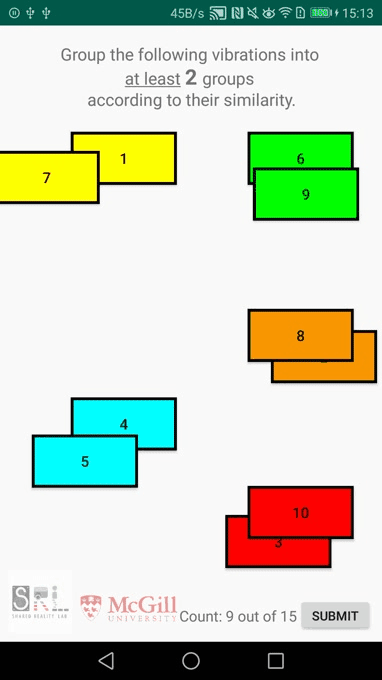
\includegraphics[width=4cm]{Images/3.png}};
            % show origin
            % \fill (0,0) circle (2pt);
            % define destination coordinates
            % \path (2.5,5.3) coordinate (im69)
            %       (2.3,1.3) coordinate (im310);
        \end{tikzpicture}
    \end{column}
\end{columns}

% define overlays
% Note the use of the overlay option. This is required when 
% you want to access nodes in different pictures.
% \begin{tikzpicture}[overlay]
        % \path[<-,green,thick] (s-69) edge [bend left] (im69);
        % \path[<-,red,thick] (s-310) edge [bend right] (im310);
% \end{tikzpicture}


\end{frame}





\begin{frame}{Logistic Model}

\begin{itemize}
    \item Logistic regression
    \begin{equation}
    \label{eqn:glm}
    P(A_i \thicksim A_j) = \hat{s}_{ij} = \frac{1}{1+e^{-(\alpha_{ij} - \alpha_{ji})}} = \frac{e^{{\alpha}_{ij}}}{e^{{\alpha}_{ij}} + e^{{\alpha}_{ji}}}, \, i<j
\end{equation}
    
    \item Variance
    \begin{equation}
\label{eqn:variance}
     \hat{\sigma}_{ij}^2 = \hat{s}_{ij} (1-\hat{s}_{ij}) = \frac{\alpha_{ij} \alpha_{ji}}{(\alpha_{ij} + \alpha_{ji})^2}
\end{equation}

    \item Maximum likelihood estimator of similarity pairs
    \begin{equation}
\label{eqn:normal_distr}
    \zeta_{ij} \sim \mathcal{N}(\hat{s}_{ij}, \hat{\sigma}_{ij})
\end{equation}

\end{itemize}
    
\end{frame}


\begin{frame}{Maximal Information Gain}

\begin{equation}
\label{eqn:eig_kld}
    U_{ij} = \infdiv{P(\zeta_{ij} \given \alpha_{ij})}{ P(\zeta_{ij}) }, \quad i<j
\end{equation}


\begin{figure}[!htb]
\centering

\begin{minipage}{.49\textwidth}
  \centering
  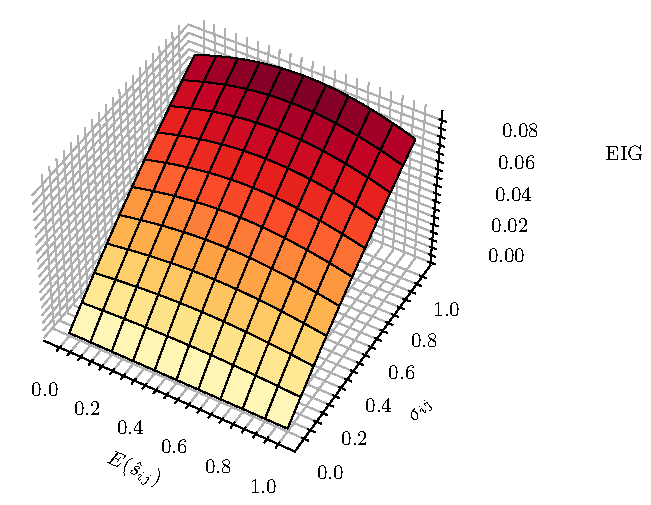
\includegraphics[width=\textwidth,keepaspectratio]{Images/EIG_3D.pdf}
%   \caption{.}
\end{minipage}%
\begin{minipage}{.49\textwidth}
  \centering
  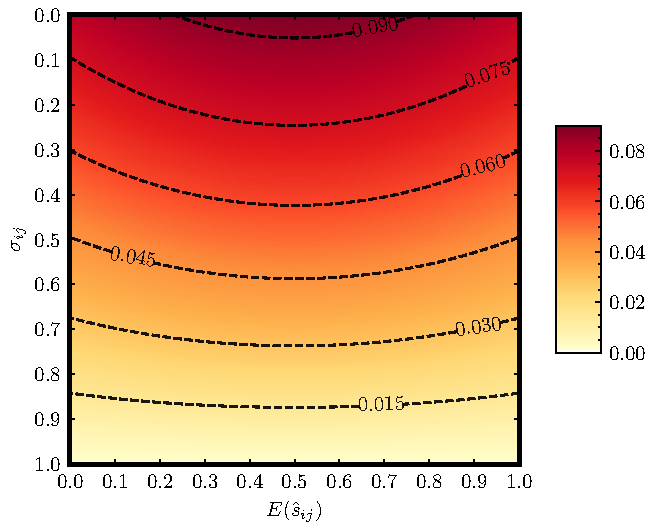
\includegraphics[width=\textwidth,keepaspectratio]{Images/EIG_2D.pdf}
%   \caption{.}
\end{minipage}
\label{fig:eig}
\end{figure}
    
\end{frame}

\begin{frame}{Representation as a Graph}

\begin{figure}[!htb]
\centering
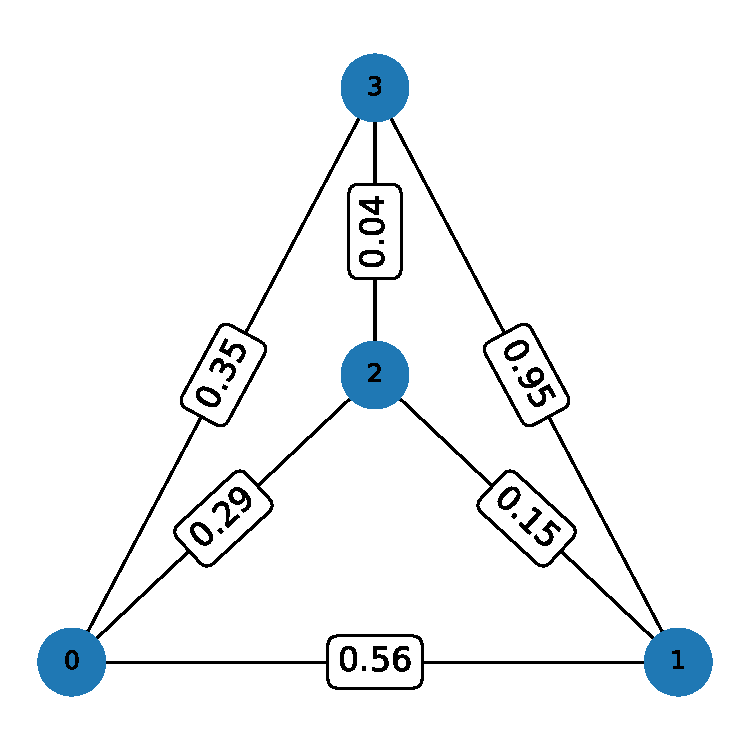
\includegraphics[width=0.4\textwidth]{Images/helper_graph.pdf}
\caption{Tacton similarity as edge weights in a graph.}
\label{fig:helper_graph}
\end{figure}
    
\end{frame}


\begin{frame}{Procedure}

We survey participants with the objective of mapping perceptual similarity in two parts:
\begin{enumerate}
    \item ``globally'': getting a consensus on what tactons are similar across a large number of tactons and of annotators.
    \item ``locally'': attempting to extract groups of people who share haptic perceptual similarity.
\end{enumerate}

\end{frame}

\begin{frame}{Procedure}

\begin{itemize}
    \item We conducted $R=8$ rounds of $c=6$ tactons each
    \item Five of those rounds were dedicated to the ``global'' experiment, while three were dedicated to the ``local'' experiment
    \item At each round the participants were asked to produce \textit{at least} two groups according to how similar they perceived the VT stimuli
    \item We allowed participants to produce singletons
\end{itemize}

\end{frame}





\section{Experimental Results}


\begin{frame}{Attention Tests}

\begin{figure}[!htb]
\centering
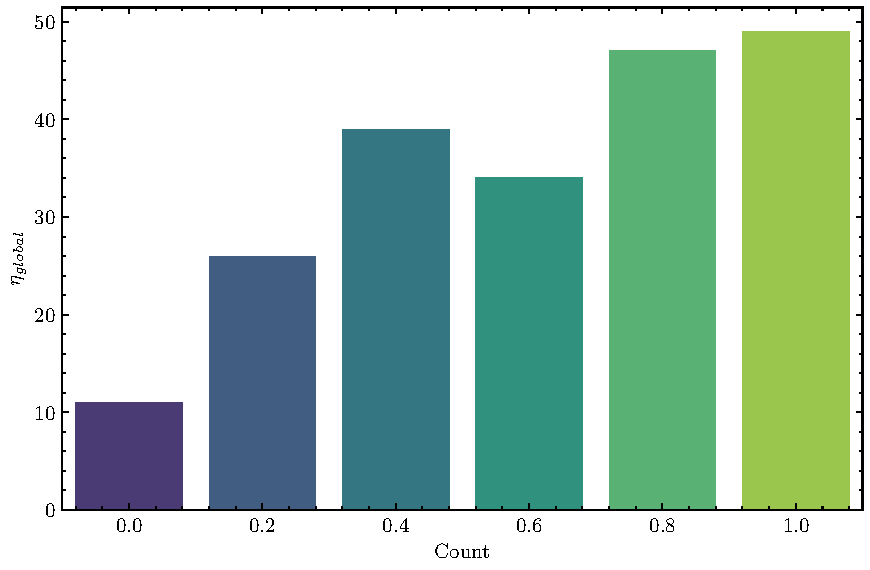
\includegraphics[width=0.5\textwidth]{Images/results_attn_tests.pdf}
\label{fig:results_attn_tests}
\end{figure}

    
\end{frame}

\begin{frame}{Active Sampling}

\begin{figure}[!htb]
\centering
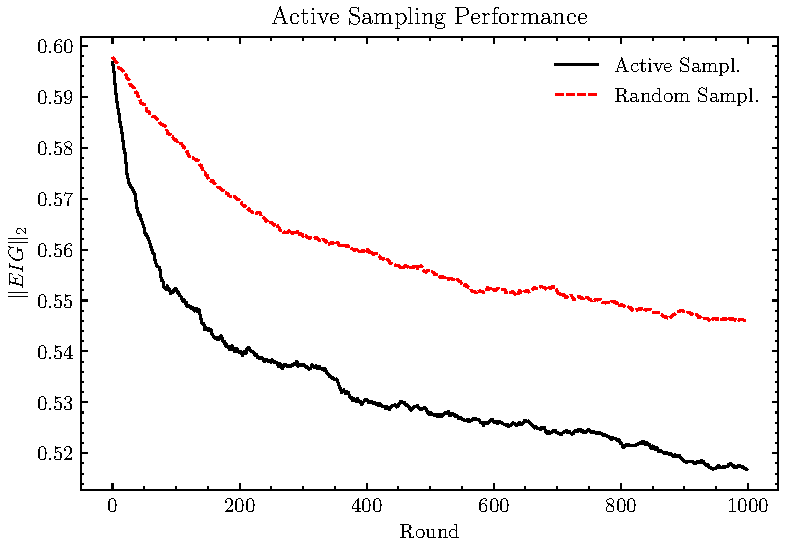
\includegraphics[width=0.5\textwidth]{Images/Active_vs_random_norm.pdf}
\label{fig:active_sampling_vs_random}
\end{figure}
    
\end{frame}

%% Results- Global

\begin{frame}{Community Detection}

\begin{figure}[!htb]
\centering
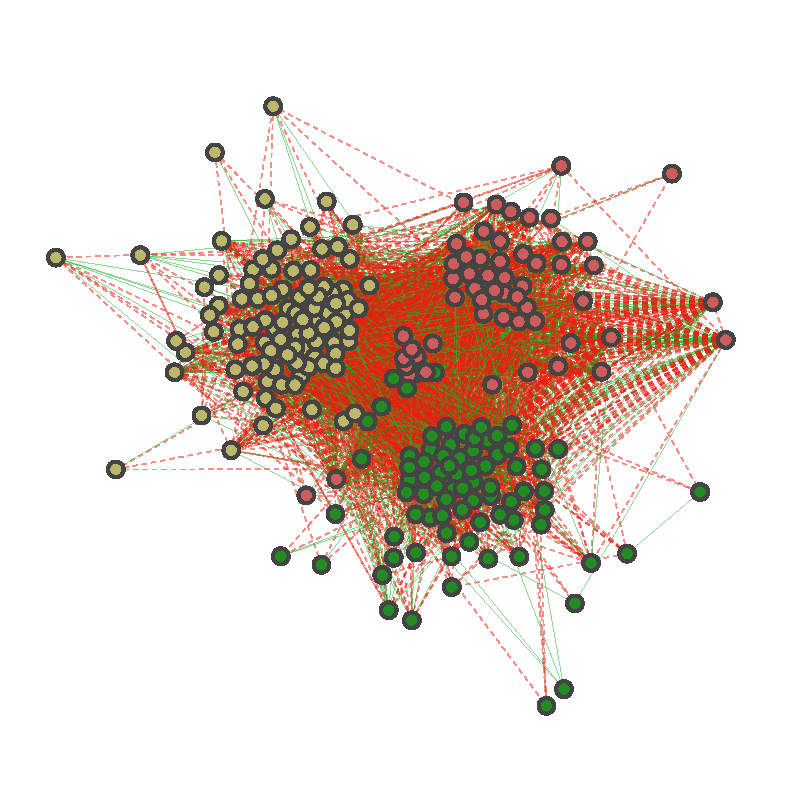
\includegraphics[width=0.6\textwidth]{Images/communities.pdf}
\label{fig:communities}
\end{figure}
    
\end{frame}


\begin{frame}{Characterizing Uncertainty Across Tactons}

\begin{figure}[!htb]
\centering
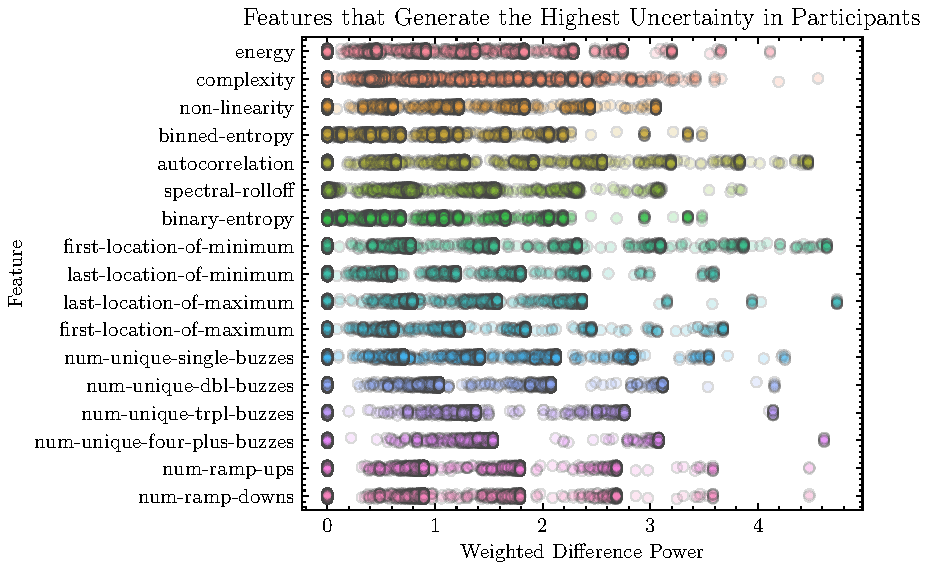
\includegraphics[width=0.8\textwidth]{Images/IDs_uncertainty.pdf}
\label{fig:ids_uncertainty}
\end{figure}
    
\end{frame}



%% Results- Personas

\begin{frame}{Personas}

\begin{figure}[!htb]
\centering
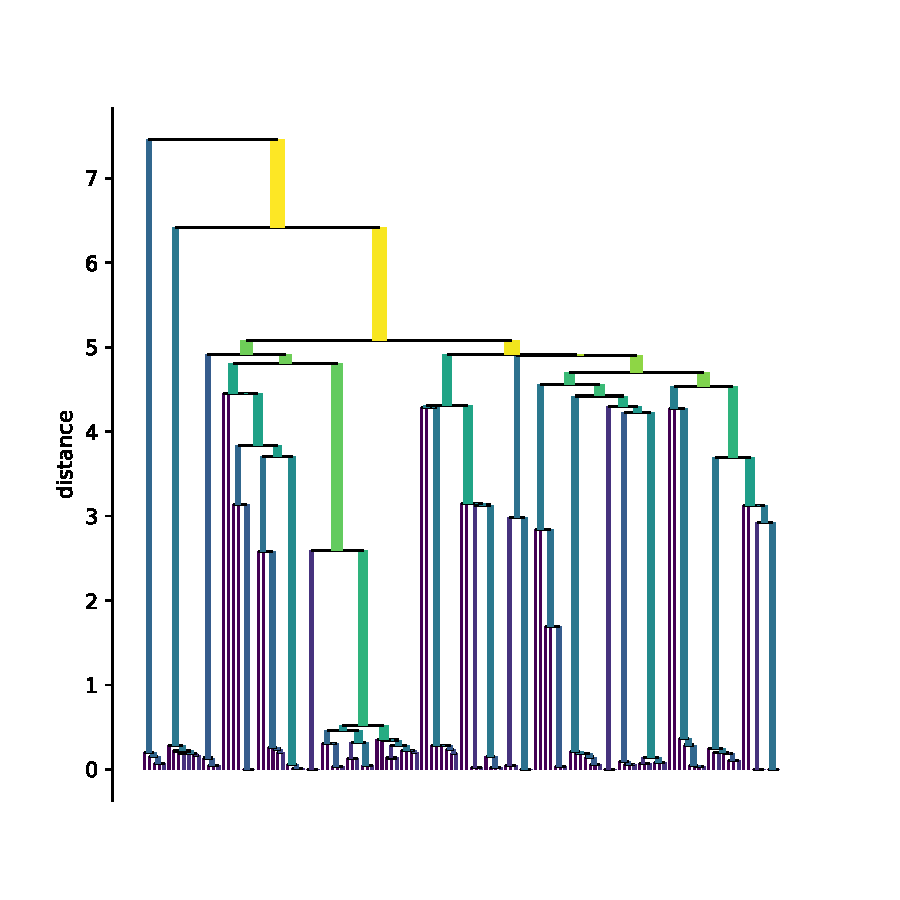
\includegraphics[width=0.6\textwidth]{Images/persona_linkage_tree.pdf}
\label{fig:persona_grouping_linkage_tree}
\end{figure}
    
\end{frame}




\begin{frame}{Demographic Information}

    \begin{figure}
\begin{subfigure}{.3\textwidth}
  \centering
  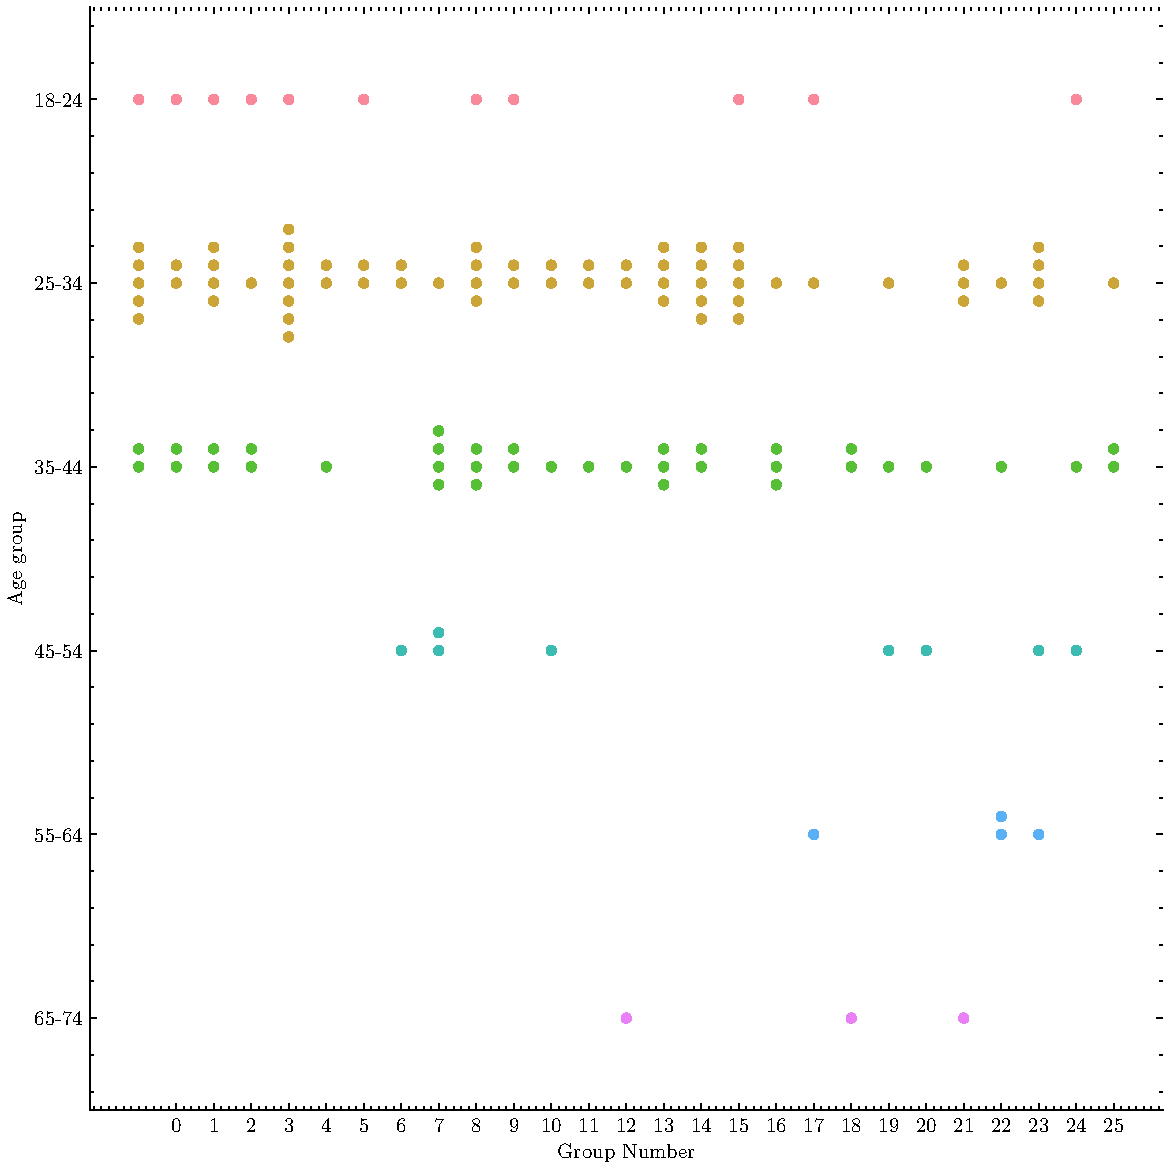
\includegraphics[width=.8\linewidth]{Images/Age_group.pdf}
  \caption{Age group}
  \label{fig:persona_age_group}
\end{subfigure}%
\begin{subfigure}{.3\textwidth}
  \centering
  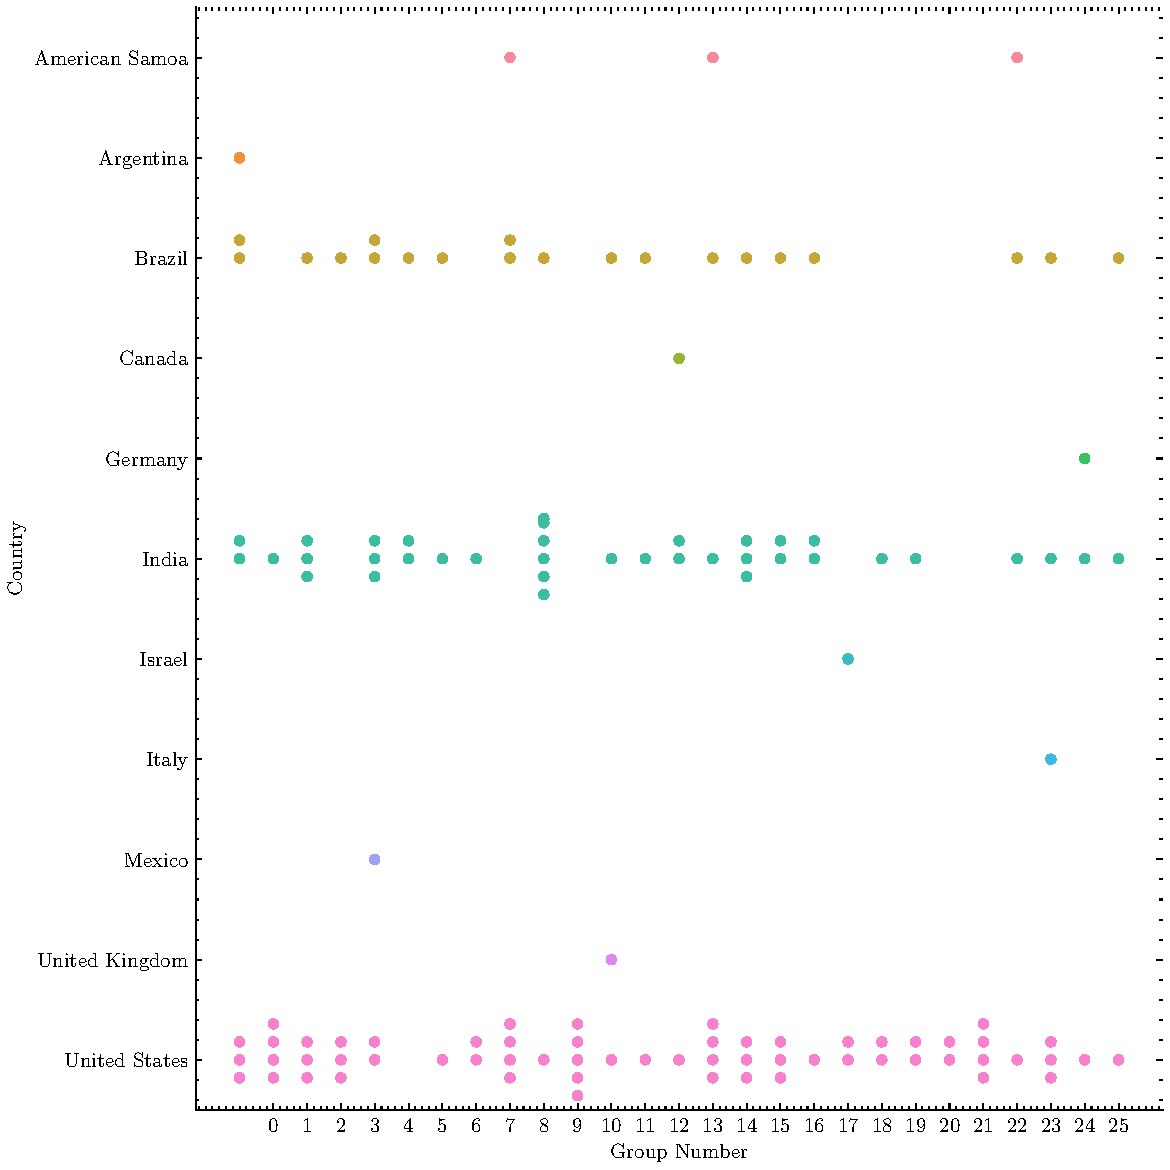
\includegraphics[width=.8\linewidth]{Images/Country.pdf}
  \caption{Country}
  \label{fig:persona_country}
\end{subfigure}
\begin{subfigure}{.3\textwidth}
  \centering
  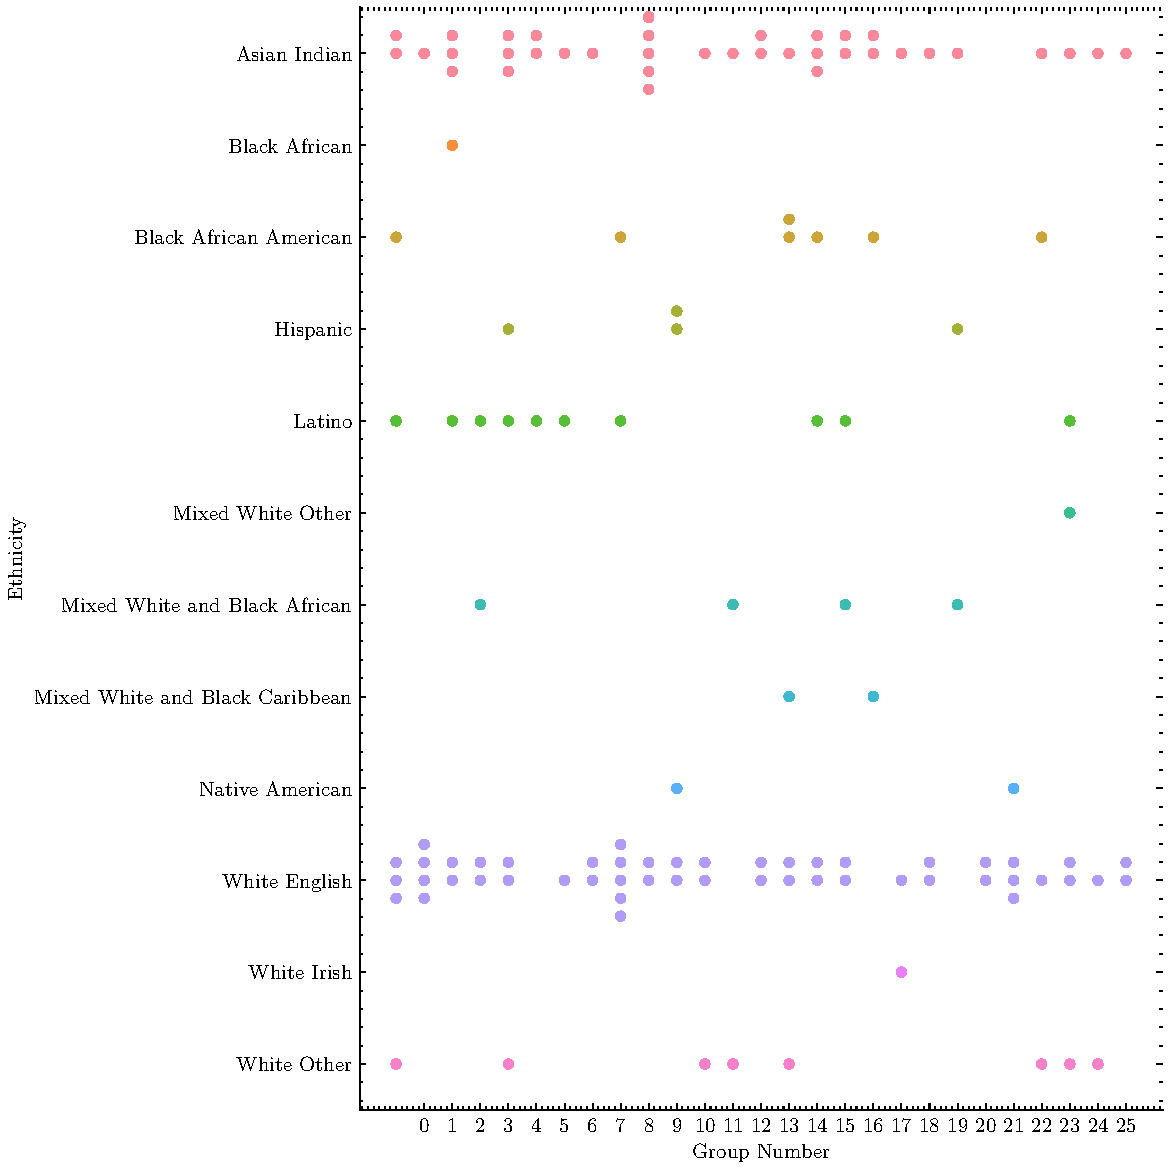
\includegraphics[width=.8\linewidth]{Images/Ethnicity.pdf}
  \caption{Ethnicity}
  \label{fig:persona_ethnicity}
\end{subfigure}
\caption{Demographic characteristics across persona groups.}
\label{fig:persona_demographic_survey}
\end{figure}

\end{frame}

\begin{frame}{Extrapolating from the Similarity Graph}

\begin{figure}[!htb]
\centering
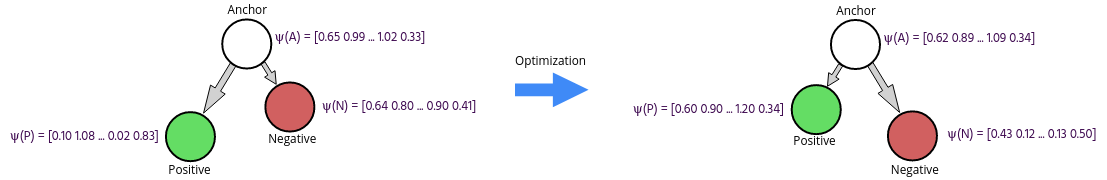
\includegraphics[width=0.9\textwidth]{Images/triplet_loss.png}
\label{fig:triplet_loss}
\end{figure}
    
\end{frame}









\begin{frame}{Learning Performance}

\begin{table}[htb]
\centering

\begin{tabular}[t]{llccc}
\toprule
 Experiment & & $R^2$ & RMSE & MAE  \\
 \midrule
 \multirow{2}{*}{All Tactons} & Lin. Reg.    & $0.081 \pm 0.042$ & $0.249 \pm 0.010$ & $0.246 \pm 0.005$ \\
 & Grad. Boost.                              & $0.152 \pm 0.012$ & $0.129 \pm 0.018$ & $0.120 \pm 0.020$ \\
 \midrule
 \multirow{2}{*}{Avg. by group} & Lin. Reg.  & $0.123 \pm 0.027$ & $0.248 \pm 0.021$ & $0.221 \pm 0.023$ \\
                            & Grad. Boost.   & $0.194 \pm 0.125$ & $0.107 \pm 0.031$ & $0.092 \pm 0.030$ \\
 \bottomrule
\end{tabular}

\label{tab:prediction_results}
\end{table}%
    
\end{frame}


\section{Conclusion}

\begin{frame}{Takeaways}

\begin{itemize}
    
    \item Provided researchers are cautious about the noise, AMT shows promise in haptic evaluation tasks
    \item The bottom-up approach proves useful in characterizing the Individual Differences on perception, something the community desperately needs
    \item It seems like there exists clusters of vibrations that users feel are similar together. Three clusters seems low but given the limited tacton space that was explored it is possible
    \item We can use machine learning to learn from similarity ratings and \textit{extrapolate} from them, which could potentially reduce the human cost of exploring the haptic tacton space
    \item Demographic info. did not seem to explain the personas
\end{itemize}
\end{frame}





\begin{frame}{TODO}

\begin{itemize}
    \item Haptics are abstract, build UI to ``feel'' the similar tactons
    \item Further analysis ideas/corrections/thoughts? 
    \item Potential reviewer for thesis
    \item Venue ideas for publishing results
\end{itemize}
    
\end{frame}





% \begin{frame}[t,allowframebreaks]
%         \frametitle{References}
% %        \bibliographystyle{amsalpha}
% \printbibliography[heading=none]
% \end{frame}


\frame[plain]{

  \centering
  \color{titlecolor}{\Large Thank you!}

}



\end{document}
